% !TEX TS-program = Xelatex
% !TEX encoding = UTF-8 Unicode

\documentclass[UTF8]{ctexart}
\usepackage{amsmath}
\usepackage[bottom]{footmisc}
\usepackage{float}
\usepackage{geometry}
\usepackage{hyperref}
\usepackage{graphicx}
\usepackage{figsize}
\usepackage[separate-uncertainty = true,per-mode=symbol]{siunitx}
\usepackage{tabu}
\usepackage{wasysym}
\geometry{left=0.7in,right=0.7in,bottom=0.7in,top=0.7in}

\title{实验二十七:交流电桥}
\author{朱寅杰 1600017721}
\date{2018年3月30日}

\begin{document}
\maketitle
\setcounter{section}{27}
实验中使用的ZX-96型电阻箱,其允差为\SI{.1}{\ohm}档2\%,\SI{1}{\ohm}档0.5\%,\SI{10}{\ohm}及以上档0.1\%。电感箱允差为2\%。电容箱100nF档允差为0.5\%,10nF档允差为0.65\%,1nF档允差为2\%,0.1nF档允差为5\%。
\subsection{测量电容器的电容与损耗电阻}
电路图如书上图27.2所示。测量时信号源频率选用$\omega/2\pi=\SI{999.35}{\Hz}$。

测量纸卷电容器时,取$R_1=R_2=\SI{600}{\ohm}$,电桥平衡时,$C_0=\SI{228.0}{\nano\F}$,$R_0=\SI{2.6}{\ohm}$,中间电表读数为\SI{.29}{mV}。那么电容和损耗电阻就分别是\SI{228.0}{nF}和\SI{2.6}{\ohm},损耗$\tan\delta=R_CC\omega=\num{3.722e-3}$。

\SI{600}{\ohm}的电阻箱允差为千分之一,\SI{228.0}{nF}的电容箱的允差为$\SI{1.29}{nF}$,\SI{2.6}{\ohm}的电阻箱的允差为\SI{.022}{\ohm}。于是电容测量值的相对不确定度为$\sqrt{2(0.1\%)^2+(1.29/228)^2}/\sqrt{3}=\num{3.37e-3}$,故电容测量值为\SI{228.0(8)}{nF};电阻测量值的相对不确定度为$\sqrt{2(0.1\%)^2+(0.022/2.6)^2}/\sqrt{3}=\num{4.95e-3}$,故电阻测量值为\SI{2.600(1)}{\ohm}。损耗角的相对不确定度也由此算出为\num{3.605e-3},损耗角为$\tan\delta=\num{3.722(13)e-3}$。

测量电解电容器时,取$R_1=\SI{500}{\ohm}$,$R_2=\SI{5}{k\ohm}$,电桥平衡时,$C_0=\SI{668.0}{\nano\F}$,$R_0=\SI{32.1}{\ohm}$,中间电表读数为\SI{.06}{mV}。那么电容和损耗电阻就分别是\SI{6680}{nF}和\SI{3.21}{\ohm},损耗$\tan\delta=R_CC\omega=\num{.1346}$。

\SI{500}{\ohm}和5k的电阻箱允差为千分之一,\SI{668.0}{nF}的电容箱的允差为$\SI{3.55}{nF}$,\SI{32.1}{\ohm}的电阻箱的允差为\SI{.042}{\ohm}。于是电容测量值的相对不确定度为$\sqrt{2(0.1\%)^2+(3.55/668.0)^2}/\sqrt{3}=\num{3.18e-3}$,故电容测量值为\SI{6.68(2)}{\micro\F};电阻测量值的相对不确定度为$\sqrt{2(0.1\%)^2+(0.042/32.1)^2}/\sqrt{3}=\num{1.11e-3}$,故电阻测量值为\SI{3.210(6)}{\ohm}。损耗角的相对不确定度也由此算出为\num{3.363e-3},损耗角为$\tan\delta=\num{.1346(5)}$。
\subsection{测量电感器的电感与电阻}
先用麦克斯韦桥测,电路图如书上图27-4所示。$L_0=\SI{6}{mH}$,$R_{L0}=\SI{4.57}{\ohm}$,$R_1=\SI{4800}{\ohm}$。电桥平衡时$R_2=\SI{4784.2}{\ohm}$,$R_0=\SI{16.4}{\ohm}$,电表读数为\SI{.99}{mV}。故电感测量值为$L_x=L_0R_1/R_2=\SI{6.0198}{mH}$,电阻为$R_L=\SI{21.039}{\ohm}$。

计算不确定度,电感箱允差为2\%;$R_1$和$R_2$都很大,允差直接按千分之一估计。合成允差时,千分之一比起百分之二忽略不计,因此电感测量值的不确定度即为$2\%/\sqrt{3}=\num{1.155e-2}$,写作$L_x=\SI{6.02(7)}{mH}$。\SI{16.4}{\ohm}的允差为\SI{.048}{\ohm},合成允差得到$R_L$的相对不确定度为\num{1.55e-3},因此写作$R_L=\SI{21.04(3)}{\ohm}$。

再用麦克斯韦-维恩桥测,电路图如书上图27-3所示。$R_1=R_2=\SI{100}{\ohm}$,电桥平衡时$R_0=\SI{469.7}{\ohm}$,$C_0=\SI{601.9}{nF}$,电表读数\SI{.16}{mV}。故电感测量值为$L_x=C_0R_1R_2=\SI{6.019}{mH}$,电阻测量值为$R_L=R_1R_2/R_0=\SI{21.29}{\ohm}$。

计算不确定度,$R_1$与$R_2$允差按千分之一计,$R_0$的允差有\SI{.519}{\ohm},$C_0$的允差有\SI{3.065}{nF}。因此$L_x=\SI{6.02(2)}{mH}$,$R_L=\SI{21.29(2)}{\ohm}$。$Q=\omega C_0R_0=\num{1.775(5)}$。

实验时二者收敛速度差不多。

\subsection{测量磁环的电感与电阻}
测量的样品是11号磁环,$D=\SI{8.56}{\cm}$,$S=\SI{2.00}{\cm^2}$,共计160匝。使用麦克斯韦-维恩桥(图27-3)进行测量,$R_1=R_2=\SI{100}{\ohm}$。数据记录见下表。
\begin{center}
\begin{tabu}{X[c]|X[c]X[c]X[c]X[c]X[c]X[c]X[c]X[c]X[c]X[c]}
\hline
$f$/kHz	&0.1&0.4&0.7&1&2&3&5&7&9&10\\
\hline
$R_0$/\si{\ohm}&6102.6&4701.6&4081.6&3707.7&3036.8&2465.8&1999.8&1957.8&1689.7&1772.6\\
$C_0$/nF&71.0&33.5&24.2&19.9&12.6&11.6&8.9&5.7&5.6&4.2\\
\hline
$L$/mH&0.710&0.335&0.242&0.199&0.126&0.116&0.089&0.057&0.056&0.042\\
$R_L$/\si{\ohm}&1.63865 &2.12694 &2.45002 &2.69709 &3.29294 &4.05548 &5.0005 &5.10777 &5.91821 &5.64143\\
\hline
$Q$&0.27224 &0.39585 &0.43443 &0.46359 &0.48084 &0.53916 &0.55915 &0.49082 &0.53508 &0.46778\\
$\mu$&29.67578 &14.00195 &10.11484 &8.31758 &5.26641 &4.84844 &3.71992 &2.38242 &2.34062 &1.75547\\
\hline
\end{tabu}
\end{center}

\begin{figure}[h]
  \centering
  \SetFigLayout{2}{1}
  \subfigure[线圈磁导率(与电感成正比)随频率的变化。]{\includegraphics[width=0.48\linewidth]{Lf.eps}}\hfill
  \subfigure[线圈的电阻与Q值随频率的变化。实线为Q值,虚线为电阻。]{\includegraphics[width=0.48\linewidth]{Qf.eps}}\\
\end{figure}

\subsection{思考题}
电桥中间的电表示数正比于$|Z_1Z_4-Z_2Z_3|$。在麦克斯韦-维恩桥中,$Z_2Z_3$是一个已知的纯电阻,调节$R_0$和$C_0$改变$Z_4$的实部和虚部即可。简单的数学计算表明控制两个参量中其中一个而改变另一个,$Z_4$会在复平面中过原点的一个圆上移动,这个圆与坐标轴相切(控制$R_0$不变则与实轴相切,控制$C_0$不变则与虚轴相切)。反复迭代调节,每次都使得$Z_4$距离目标点最近就行。
\end{document} 